\documentclass[12pt,a4paper]{article}
\usepackage{amsmath,amssymb,mathrsfs,tikz,times,pifont}
\usepackage{enumitem}
\newcommand\circitem[1]{%
\tikz[baseline=(char.base)]{
\node[circle,draw=gray, fill=red!55,
minimum size=1.2em,inner sep=0] (char) {#1};}}
\newcommand\boxitem[1]{%
\tikz[baseline=(char.base)]{
\node[fill=cyan,
minimum size=1.2em,inner sep=0] (char) {#1};}}
\setlist[enumerate,1]{label=\protect\circitem{\arabic*}}
\setlist[enumerate,2]{label=\protect\boxitem{\alph*}}
%%%::::::by chnini ameur :::::::%%%
\everymath{\displaystyle}
\usepackage[left=1cm,right=1cm,top=1cm,bottom=1.7cm]{geometry}
\usepackage{array,multirow}
\usepackage[most]{tcolorbox}
\usepackage{varwidth}
\usepackage{tkz-tab}
\tcbuselibrary{skins,hooks}
\usetikzlibrary{patterns}
%%%::::::by chnini ameur :::::::%%%
\newtcolorbox{exa}[2][]{enhanced,breakable,before skip=2mm,after skip=5mm,
colback=yellow!20!white,colframe=black!20!blue,boxrule=0.5mm,
attach boxed title to top left ={xshift=0.6cm,yshift*=1mm-\tcboxedtitleheight},
fonttitle=\bfseries,
title={#2},#1,
% varwidth boxed title*=-3cm,
boxed title style={frame code={
\path[fill=tcbcolback!30!black]
([yshift=-1mm,xshift=-1mm]frame.north west)
arc[start angle=0,end angle=180,radius=1mm]
([yshift=-1mm,xshift=1mm]frame.north east)
arc[start angle=180,end angle=0,radius=1mm];
\path[left color=tcbcolback!60!black,right color = tcbcolback!60!black,
middle color = tcbcolback!80!black]
([xshift=-2mm]frame.north west) -- ([xshift=2mm]frame.north east)
[rounded corners=1mm]-- ([xshift=1mm,yshift=-1mm]frame.north east)
-- (frame.south east) -- (frame.south west)
-- ([xshift=-1mm,yshift=-1mm]frame.north west)
[sharp corners]-- cycle;
},interior engine=empty,
},interior style={top color=yellow!5}}
%%%%%%%%%%%%%%%%%%%%%%%

\usepackage{fancyhdr}
\usepackage{eso-pic}         % Pour ajouter des éléments en arrière-plan
% Commande pour ajouter du texte en arrière-plan
\AddToShipoutPicture{
    \AtTextCenter{%
        \makebox[0pt]{\rotatebox{80}{\textcolor[gray]{0.7}{\fontsize{5cm}{5cm}\selectfont PGB}}}
    }
}
\usepackage{lastpage}
\fancyhf{}
\pagestyle{fancy}
\renewcommand{\footrulewidth}{1pt}
\renewcommand{\headrulewidth}{0pt}
\renewcommand{\footruleskip}{10pt}
\fancyfoot[R]{
\color{blue}\ding{45}\ \textbf{2025}
}
\fancyfoot[L]{
\color{blue}\ding{45}\ \textbf{Prof:M. BA}
}
\cfoot{\bf
\thepage /
\pageref{LastPage}}
\begin{document}
\renewcommand{\arraystretch}{1.5}
\renewcommand{\arrayrulewidth}{1.2pt}
\begin{tikzpicture}[overlay,remember picture]
\node[draw=blue,line width=1.2pt,fill=purple,text=blue,inner sep=3mm,rounded corners,pattern=dots]at ([yshift=-2.5cm]current page.north) {\begingroup\setlength{\fboxsep}{0pt}\colorbox{white}{\begin{tabular}{|*1{>{\centering \arraybackslash}p{0.28\textwidth}} |*2{>{\centering \arraybackslash}p{0.2\textwidth}|} *1{>{\centering \arraybackslash}p{0.19\textwidth}|} }
\hline
\multicolumn{3}{|c|}{$\diamond$$\diamond$$\diamond$\ \textbf{Lycée de Dindéfélo}\ $\diamond$$\diamond$$\diamond$ }& \textbf{A.S. : 2024/2025} \\ \hline
\textbf{Matière: Mathématiques}& \textbf{Niveau : T}\textbf{S2} &\textbf{Date: 21/01/2025} & \textbf{Durée : 4 heures} \\ \hline
\multicolumn{4}{|c|}{\parbox[c]{10cm}{\begin{center}
\textbf{{\Large\sffamily Correction Devoir n$ ^{\circ} $ 2 Du 1$ ^\text{\bf er} $ Semestre}}
\end{center}}} \\ \hline
\end{tabular}}\endgroup};
\end{tikzpicture}
\vspace{3cm}

\section*{\underline{Exercice 1 :} 4 points [\textit{ Déjà corrigé en classe}]}
Soit \((u_n)_{n \in \mathbb{N}^*}\) la suite numérique définie par :
\[
\begin{cases}
u_1 = \frac{1}{3}, \\
(\forall n \in \mathbb{N}^*), \ u_{n+1} = \frac{2u_n}{1 + (n+2)u_n}.
\end{cases}
\]

Soit \((v_n)_{n \in \mathbb{N}^*}\) la suite numérique définie par : \(v_n = \frac{1}{u_n} - n\).

\begin{enumerate}
    \item Montrer que la suite \((v_n)_{n \in \mathbb{N}^*}\) est géométrique.\hfill \textbf{1,5 pt}

    \item 
    \begin{enumerate}
        \item Déterminer \(v_n\) et \(u_n\) en fonction de \(n\).\hfill \textbf{1 pt}
        \item Calculer en fonction de \(n\) la somme : \(S_n = v_1 + v_2 + \cdots + v_n\).\hfill \textbf{1,5 pt}
    \end{enumerate}
\end{enumerate}
\section*{\textcolor{green}{\underline{Correction Exercice 1 :} 4 points [\textit{ Déjà corrigé en classe}]}}
Soit \((u_n)_{n \in \mathbb{N}^*}\) la suite numérique définie par :
\[
\begin{cases}
u_1 = \frac{1}{3}, \\
(\forall n \in \mathbb{N}^*), \ u_{n+1} = \frac{2u_n}{1 + (n+2)u_n}.
\end{cases}
\]

Soit \((v_n)_{n \in \mathbb{N}^*}\) la suite numérique définie par : \(v_n = \frac{1}{u_n} - n\).

\begin{enumerate}
    \item Montrons que la suite \((v_n)_{n \in \mathbb{N}^*}\) est géométrique.\hfill \textbf{1,5 pt}
    
\((v_n)\) est une suite géométrique ssi $\frac{v_{n+1}}{v_n}=q \in \mathbb{R}^{*}\setminus\{1\}$

In fact : \\
$
\begin{aligned}
\frac{v_{n+1}}{v_n}&=\frac{\frac{1}{u_{n+1}} - (n+1)}{\frac{1}{u_n} - n}\\
									&=\frac{\frac{1}{\frac{2u_n}{1 + (n+2)u_n}} - (n+1)}{\frac{1 - nu_n}{u_n}}\\
									&=\frac{\frac{{1 + (n+2)u_n}}{2u_n} - (n+1)}{\frac{1 - nu_n}{u_n}}\\
									&=\frac{\frac{1 + (n+2)u_n - (n+1)2u_n}{2u_n}}{\frac{1 - nu_n}{u_n}}\\
									&=\frac{\frac{1 + nu_n+2u_n - n2u_n-2u_n}{2u_n}}{\frac{1 - nu_n}{u_n}}\\
									&=\frac{1 + nu_n+2u_n - n2u_n-2u_n}{2(1 - nu_n)}\\
									&=\frac{1 - nu_n}{2(1 - nu_n)}\\
									&=\frac{1}{2}\\
\end{aligned}
$

\text{ Donc \(v_n\) est une suite gémétrique de raison \(\frac{1}{2}\) et de premier terme:} 
\( v_1 = \frac{1}{u_1} - 1=\frac{1}{\frac{1}{3}} - 1=3 - 1 =2 \)    
    \item 
    \begin{enumerate}
        \item Déterminons \(v_n\) et \(u_n\) en fonction de \(n\).\hfill \textbf{1 pt}
        
        \((v_n)\) est une suite géométrique donc \(v_n=v_p \times q^{n-p}\)
        
        Ainsi: \(v_n=2 \times \left( \frac{1}{2}\right)^{n-1}\)
        
        \(\boxed{\textcolor{green}{v_n=2 \times \left( \frac{1}{2}\right)^{n-1}}}\)
        
        On a \(v_n = \frac{1}{u_n} - n\) donc \(u_n = \frac{1}{v_n + n}\)
        
        Ainsi: \(u_n = \frac{1}{2 \times \left( \frac{1}{2}\right)^{n-1} + n}\)
        \item Calculer en fonction de \(n\) la somme : \(S_n = v_1 + v_2 + \cdots + v_n\).\hfill \textbf{1,5 pt}
        
        \(
        \begin{aligned}
        S_n = v_1 + v_2 + \cdots + v_n &= v_1 \times \frac{1-\left( \frac{1}{2}\right)^{n-1+1} }{1-\frac{1}{2}}\\
										&=2 \times \frac{1-\left( \frac{1}{2}\right)^{n} }{\frac{1}{2}}\\ 
										&=4 \times \left[ 1-\left( \frac{1}{2}\right)^{n}\right] \\     
        \end{aligned}
        \)
        
        \(\boxed{\textcolor{green}{S_n=4 \times \left[ 1-\left( \frac{1}{2}\right)^{n}\right]}}\)
    \end{enumerate}
\end{enumerate}
\section*{\underline{Exercice 2 (BAC 2022) :} 4 points [\textit{ Déjà corrigé en classe par moi-même}]}
Le plan complexe est muni d’un repère orthonormé direct $(O; \vec{u}, \vec{v})$. Soit le nombre complexe $a$ défini par 
\[
a = \sqrt{2 - \sqrt{3}} - i\sqrt{2 + \sqrt{3}}.
\]

\begin{enumerate}
    \item Montrer que $a^2 = -2\sqrt{3} - 2i$, puis en déduire le module de $a$. \hfill \textbf{0,5 + 0,5 pt}

    \item Écrire $a^2$ sous forme trigonométrique puis \\vérifier qu’une des mesures de l’argument de $a$ est $\frac{19\pi}{12}$. \hfill \textbf{0,5 + 0,5 pt}

    \item En déduire les valeurs exactes de $\cos\left(\frac{7\pi}{12}\right)$ et $\sin\left(\frac{7\pi}{12}\right)$, puis de $\cos\left(\frac{\pi}{12}\right)$ et $\sin\left(\frac{\pi}{12}\right)$. \hfill \textbf{1 pt}

    \item Représenter sur le même graphique les points images de $a$, $-a$ et $a^2$. \hfill \textbf{1 pt}
\end{enumerate}
\section*{\textcolor{green}{\underline{Correction Exercice 2 (BAC 2022) :} 4 points [\textit{ Déjà corrigé en classe par moi-même}]}}
Le plan complexe est muni d’un repère orthonormé direct $(O; \vec{u}, \vec{v})$. Soit le nombre complexe $a$ défini par 
\[
a = \sqrt{2 - \sqrt{3}} - i\sqrt{2 + \sqrt{3}}.
\]

\begin{enumerate}
    \item Montrons que $a^2 = -2\sqrt{3} - 2i$. \hfill \textbf{0,5}
    
     On a : \\
     $
     \begin{aligned}
     a^{2} &= \left( \sqrt{2 - \sqrt{3}} - i\sqrt{2 + \sqrt{3}}\right)^{2}\\
     &=\left( \sqrt{2 - \sqrt{3}}\right)^{2} -2i\sqrt{2 - \sqrt{3}}\sqrt{2 + \sqrt{3}} + \left( i\sqrt{2 + \sqrt{3}}\right)^{2}\\
     &=\left( 2 - \sqrt{3} \right) -2i\sqrt{\left( 2 - \sqrt{3} \right)\left( 2 + \sqrt{3}\right)} - \left( 2 + \sqrt{3}\right)\\
     &=\left( 2 - \sqrt{3} \right)  - \left( 2 + \sqrt{3}\right)-2i\sqrt{ 2^{2} - \sqrt{3}^{2}}\\
     &= 2 - \sqrt{3}   -  2 - \sqrt{3}-2i\sqrt{4 - 3}\\
     &= - \sqrt{3} - \sqrt{3}-2i\sqrt{1}\\
     &= -2\sqrt{3}-2i\\
     \end{aligned}
     $
     
     Donc $\textcolor{green}{\underline{a^2 = -2\sqrt{3} - 2i}} \text{ cqfd}$

	Déduisons-en le module de $a$ \hfill \textbf{0,5}
	
	On a $a^2 = -2\sqrt{3} - 2i$ donc $|a^2|=\sqrt{(-2\sqrt{3})^{2} + (-2)^{2} } \implies |a^2|=4$
	
	$|a^2|=4 \implies |a^2|=|a|^2=2^{2} \implies |a|=2$
	
	Donc $\textcolor{green}{\underline{|a|=2}} $
    \item Écrivons $a^2$ sous forme trigonométrique \hfill \textbf{0,5}
    
     $
     \begin{aligned}
     a^2&= -2\sqrt{3}-2i\\
     	&=4\left(\frac{-\sqrt{3}}{2}-i\frac{1}{2}\right)\\
     	&=4\left[ \cos\left( \frac{7\pi}{6}\right) +i\sin\left( \frac{7\pi}{6}\right)  \right]
     \end{aligned}
     $
     
     Donc $\textcolor{green}{\underline{a^2 = 4\left[ \cos\left( \frac{7\pi}{6}\right) +i\sin\left( \frac{7\pi}{6}\right)  \right]}} $
     
    Vérifions qu’une des mesures de l’argument de $a$ est $\frac{19\pi}{12}$. \hfill \textbf{0,5}
    
    On a :
     
     $
     \begin{aligned}
		\arg(a^2)&=\frac{7\pi}{6}[2\pi]\\
		2\arg(a)&=\frac{7\pi}{6}[2\pi]\\
		\arg(a)&=\frac{7\pi}{12}[\pi]\\
     \end{aligned}
     $

$ \arg(a)=\frac{7\pi}{12}[\pi] \Leftrightarrow \arg(a)=\frac{7\pi}{12}+k\pi $

Si $k=1$ on a : $\arg(a)=\frac{19\pi}{12}$
    \item Déduison-en les valeurs exactes de $\cos\left(\frac{7\pi}{12}\right)$ et $\sin\left(\frac{7\pi}{12}\right)$

	    On a : $ \arg(a)=\frac{19\pi}{12} $ donc 
	    $
	    \begin{cases}
	    \cos\left(\frac{19\pi}{12}\right)=\frac{\sqrt{2 - \sqrt{3}}}{2}\\
	    \sin\left(\frac{19\pi}{12}\right)=-\frac{\sqrt{2 + \sqrt{3}}}{2}
	    \end{cases}
	     $
	     
	Or $\frac{19\pi}{12}=\frac{7\pi+12\pi}{12}=\frac{7\pi}{12}+\pi$
	
	  donc  $
	    \begin{cases}
	    \cos\left(\frac{19\pi}{12}\right)=\frac{\sqrt{2 - \sqrt{3}}}{2}\\
	    \sin\left(\frac{19\pi}{12}\right)=-\frac{\sqrt{2 + \sqrt{3}}}{2}
	    \end{cases}\implies
	    \begin{cases}
	    \cos\left(\frac{7\pi}{12}+\pi\right)=\frac{\sqrt{2 - \sqrt{3}}}{2}\\
	    \sin\left(\frac{7\pi}{12}+\pi\right)=-\frac{\sqrt{2 + \sqrt{3}}}{2}
	    \end{cases}
	    $
	    
		$
		\begin{cases}
	    -\cos\left(\frac{7\pi}{12}\right)=\frac{\sqrt{2 - \sqrt{3}}}{2}\\
	    -\sin\left(\frac{7\pi}{12}\right)=-\frac{\sqrt{2 + \sqrt{3}}}{2}
	    \end{cases}\implies
	   	\begin{cases}
	    \cos\left(\frac{7\pi}{12}\right)=-\frac{\sqrt{2 - \sqrt{3}}}{2}\\
	    \sin\left(\frac{7\pi}{12}\right)=\frac{\sqrt{2 + \sqrt{3}}}{2}
	    \end{cases}
	    $    \hfill \textbf{0,5 pt}
	    
    \[\boxed{\textcolor{green}{\begin{cases}
	    \cos\left(\frac{7\pi}{12}\right)=-\frac{\sqrt{2 - \sqrt{3}}}{2}\\
	    \sin\left(\frac{7\pi}{12}\right)=\frac{\sqrt{2 + \sqrt{3}}}{2}
	    \end{cases}}}\]

    Puis les valeurs exactes de $\cos\left(\frac{\pi}{12}\right)$ et $\sin\left(\frac{\pi}{12}\right)$. \hfill \textbf{0,5 pt}
	     
	Or $\frac{7\pi}{12}=\frac{6\pi+\pi}{12}=\frac{\pi}{12}+\frac{\pi}{2}$
	
	  donc  $
		\begin{cases}
	    \cos\left(\frac{7\pi}{12}\right)=-\frac{\sqrt{2 - \sqrt{3}}}{2}\\
	    \sin\left(\frac{7\pi}{12}\right)=\frac{\sqrt{2 + \sqrt{3}}}{2}
	    \end{cases}\implies
	    \begin{cases}
	    \cos\left(\frac{\pi}{12}+\frac{\pi}{2}\right)=-\frac{\sqrt{2 - \sqrt{3}}}{2}\\
	    \sin\left(\frac{\pi}{12}+\frac{\pi}{2}\right)=\frac{\sqrt{2 + \sqrt{3}}}{2}
	    \end{cases}
	    $
	    
		$
		\begin{cases}
	    -\sin\left(\frac{\pi}{12}\right)=-\frac{\sqrt{2 - \sqrt{3}}}{2}\\
	    \cos\left(\frac{\pi}{12}\right)=\frac{\sqrt{2 + \sqrt{3}}}{2}
	    \end{cases}\implies
	   	\begin{cases}
	    \sin\left(\frac{\pi}{12}\right)=\frac{\sqrt{2 - \sqrt{3}}}{2}\\
	    \cos\left(\frac{\pi}{12}\right)=\frac{\sqrt{2 + \sqrt{3}}}{2}
	    \end{cases}
	    $
	    
    \[\boxed{\textcolor{green}{\begin{cases}
	    \cos\left(\frac{\pi}{12}\right)=\frac{\sqrt{2 + \sqrt{3}}}{2}\\
	    \sin\left(\frac{\pi}{12}\right)=\frac{\sqrt{2 - \sqrt{3}}}{2}
	    \end{cases}}}\]    \hfill \textbf{0,5 pt}
    \item Représentons sur le même graphique les points images de $a$, $-a$ et $a^2$. \hfill \textbf{1 pt}
    
    \begin{center}
    \includegraphics[width=0.5\textwidth]{devoir2.png}
\end{center}

NB ici $z_{1}=-a$ et $b=a^{2}$
\end{enumerate}
\section*{\underline{Exercice 3 :} 4 points [\textit{ Exercice 1  du devoir N1 déjà  corrigé par moi-même}]}

\begin{enumerate}
    \item Calculer les limites suivantes :\hfill \textbf{( 0,5pt $\times$ 3+0,25pt )}
    \[
    \lim_{x \to 0} \frac{\sqrt{1+\sin x} - 1}{\sin 2x} \; ; \quad
    \lim_{x \to 0} \frac{\cos x - 1}{x^3 + x^2} \; ; \quad
    \lim_{x \to 1} \frac{\sqrt{x + 3} - \sqrt{5 - x}}{\sqrt{2x + 7} - \sqrt{10 - x}}.
    \]
    \item Donner les primitives des fonctions \(f\) et \(g\) respectivement sur \(\mathbb{R}\) et \(\mathbb{R} \setminus \{1; 2\}\).\hfill \textbf{(2 × 0,5 pt)}
    \[
    f(x) = (3x-1)(3x^2-2x+3)^3 \; ; \quad
    g(x) = \frac{1-x^2}{(x^3-3x+2)^3}.
    \]
\end{enumerate}

\section*{\textcolor{green}{\underline{Correction 3 :} 4 pts [\textit{ Exercice 1  du devoir N1 déjà  corrigé par moi-même}]}}
\begin{enumerate}
    \item Calculons les limites suivantes : \textbf{(3 × 1 pt)}
    \begin{align*}
    \lim_{x \to 0} \frac{\sqrt{1+\sin x} - 1}{\sin 2x}&=\lim_{x \to 0} \frac{\sin x }{\sin 2x\left( \sqrt{1+\sin x} + 1\right) }\\
    &=\lim_{x \to 0} \frac{\frac{\sin x}{x} }{\frac{2\sin 2x}{2x}}\times \frac{1}{\left(\sqrt{1+\sin x} + 1\right)}\\
    &=\frac{1}{2}\times\frac{1}{2}\\
    &=\frac{1}{4}
    \end{align*}
\[
\textcolor{green}{\boxed{ \lim_{x \to 0} \frac{\sqrt{1+\sin x} - 1}{\sin 2x}=\frac{1}{4}  }} \textbf{ 0,25 points}
\]

    \begin{align*}
    \lim_{x \to 0} \frac{\cos x - 1}{x^3 + x^2}&=\lim_{x \to 0}\frac{\cos x - 1}{x^2(x + 1)}\\
    &=\lim_{x \to 0} \frac{\cos x - 1}{x^{2}} \times \frac{1}{x+1}\\
    &=-\frac{1}{2}\times1\\
    &=-\frac{1}{2}
    \end{align*}
\[
\textcolor{green}{\boxed{ \lim_{x \to 0} \frac{\cos x - 1}{x^3 + x^2}=-\frac{1}{2}  }} \textbf{ 0,25 points}
\]

    \begin{align*}
    \lim_{x \to 1} \frac{\sqrt{x + 3} - \sqrt{5 - x}}{\sqrt{2x + 7} - \sqrt{10 - x}}&=\lim_{x \to 0}\frac{\left( \sqrt{x + 3} - \sqrt{5 - x}\right)\left( \sqrt{x + 3} + \sqrt{5 - x}\right)\left( \sqrt{2x + 7} - \sqrt{10 - x}\right) }{\left( \sqrt{2x + 7} - \sqrt{10 - x}\right) \left( \sqrt{2x + 7} - \sqrt{10 - x}\right) \left( \sqrt{x + 3} - \sqrt{5 - x}\right)}\\
    &=\lim_{x \to 1} \frac{\left[ x + 3 - (5 - x)\right]\left( \sqrt{2x + 7} + \sqrt{10 - x}\right) }{ \left[  2x + 7 - (10 - x) \right]  \left( \sqrt{x + 3} + \sqrt{5 - x}\right)}\\
    &=\lim_{x \to 1} \frac{2(-1+x)\left( \sqrt{2x + 7} + \sqrt{10 - x}\right) }{ 3( x - 1 )  \left( \sqrt{x + 3} + \sqrt{5 - x}\right)}\\
    &=\lim_{x \to 1} \frac{2(x-1)\left( \sqrt{2x + 7} + \sqrt{10 - x}\right) }{ 3( x - 1 )  \left( \sqrt{x + 3} + \sqrt{5 - x}\right)}\\
    &=\lim_{x \to 1} \frac{2\left( \sqrt{2x + 7} + \sqrt{10 - x}\right) }{ 3\left( \sqrt{x + 3} + \sqrt{5 - x}\right)}\\
    &=\frac{2}{3} \times \frac{6}{4}
    \end{align*}
\[
\textcolor{green}{\boxed{ \lim_{x \to 1} \frac{\sqrt{x + 3} - \sqrt{5 - x}}{\sqrt{2x + 7} - \sqrt{10 - x}}=1 }} \textbf{ 0,25 points}
\]
    \item Donnons les primitives des fonctions \(f\) et \(g\) respectivement sur \(\mathbb{R}\) et \(\mathbb{R} \setminus \{1; 2\}\). \textbf{(2 × 0,5 pt)}
    \[
    f(x) = (3x-1)(3x^2-2x+3)^3 
    \]

		\[
    F(x) =\frac{1}{8}(3x^2-2x+3)^4+k
    \] 
       
    \[
     \textcolor{green}{\boxed{ \lim_{x \to 1} F(x) =\frac{1}{8}(3x^2-2x+3)^4 + k }} \textbf{ 0,25 points}
    \]
    
    \[
    g(x) = \frac{1-x^2}{(x^3-3x+2)^3}.
    \]
    
    \[
     \textcolor{green}{\boxed{ \lim_{x \to 1} G(x) = \frac{1}{3(x^3-3x+2)} + k }} \textbf{ 0,25 points}
    \]
\end{enumerate}
\section*{\underline{Problème :} 9,75 points [\textit{ Exercice d'application déjà corrigé par moi-même}]} 

Soit $f$ la fonction définie par :
\[
f(x) =
\begin{cases} 
2x\sqrt{1 - x^2} & \text{si } x > 0 \\ 
-x + \sqrt{x^2 - 2x} & \text{si } x \leq 0 
\end{cases}
\]

\begin{enumerate}
    \item Déterminer $D_f$, les limites aux bornes et préciser la branche infinie.\hfill \textbf{( 0,5pt $\times$ 3)}
    \item Étudier la dérivabilité de $f$ en 0 et 1\\interpréter géométriquement les résultats obtenus.\hfill \textbf{( 0,5pt $\times$ 3+0,5pt $\times$ 3 )}
    \item Calculer $f'(x)$ là où $f$ est définie, puis dresser le tableau de variation de $f$.\hfill \textbf{( 0,5pt $\times$ 2+0,5pt $\times$ 2 + 0,5pt )}
    \item Tracer la courbe de $f$.\hfill \textbf{( 0,75pt )}
    \item Soit $h$ la restriction de $f$ à l’intervalle $]-\infty ; 0]$.
    \begin{enumerate}
        \item Montrer que $h$ admet une bijection réciproque $h^{-1}$ dont on précisera l’ensemble de définition, l’ensemble de dérivabilité et le tableau de variation.\hfill \textbf{( 0,5pt )}
        \item Sans utiliser l’expression de $h^{-1}(x)$, calculer $(h^{-1})'(2)$.\hfill \textbf{( 0,5pt )}
        \item Déterminer explicitement $h^{-1}$.\hfill \textbf{( 0,5pt )}
        \item Tracer la courbe de $h^{-1}$ dans le même repère que celle de $f$.\hfill \textbf{( 0,5pt )}
    \end{enumerate}
\end{enumerate}
\section*{\textcolor{green}{\underline{Problème :} 9,75 pts [\textit{ Exercice d'application déjà corrigé par moi-même}]}}
Soit $f$ la fonction définie par :
\[
f(x) =
\begin{cases} 
2x\sqrt{1 - x^2} & \text{si } x > 0 \\ 
-x + \sqrt{x^2 - 2x} & \text{si } x \leq 0 
\end{cases}
\]
\begin{enumerate}
\item Déterminer $D_f$, les limites aux bornes et préciser la branche infinie.\hfill \textbf{( 0,5pt $\times$ 3)}
\[\text{Posons }
f(x) =
\begin{cases} 
f_1(x) & \text{si } x > 0, \\ 
f_2(x) & \text{si } x \leq 0.
\end{cases}
\]

\( \bullet \) \(f_1 \exists \text{ ssi } 1 - x^2 \geq 0 \text{ et } x > 0. \)

\(\text{ Posnos } 1 - x^2 = 0 \text{ et } x = 0. \)

\( 1 - x^2 = 0 \text{ et } x = 0 \implies x = -1 \text{ ou } x = 1 \text{ et } x = 0 \)

    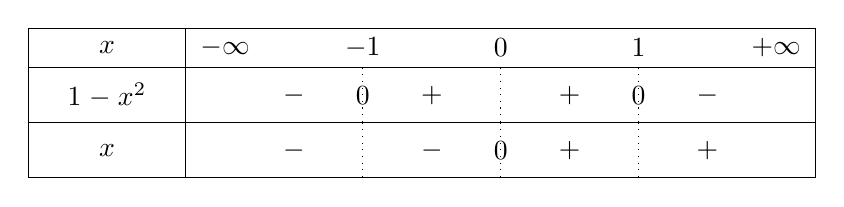
\begin{tikzpicture}[node style/.style={fill opacity=0,text opacity=1}]
        \tkzTabInit[espcl=1.75]
        {$x$/.5, $1 - x^2$/.7, $x$/.7}
        {$-\infty$,$-1$,$0$,$1$,$+\infty$}
        \tkzTabLine{,-,z,+,t,+,z,-}
        \tkzTabLine{,-,t,-,z,+,t,+}
    \end{tikzpicture}
    
    \underline{\( Df_1 = ]0;1] \)}
    
\( \bullet \) \(f_1 \exists \text{ ssi } x^2 - x \geq 0 \text{ et } x \leq 0. \) 

\(\text{ Posnos } x^2 - x = 0 \text{ et } x = 0. \)

\( x^2 - x = 0 \text{ et } x = 0 \implies x = 0 \text{ ou } x = 1 \text{ et } x = 0 \)  

    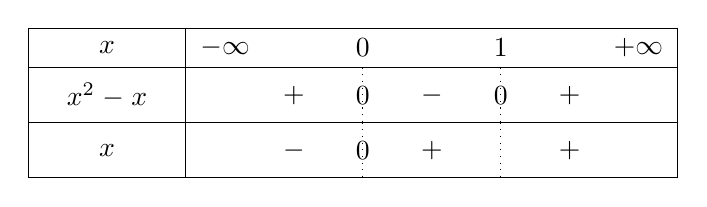
\begin{tikzpicture}[node style/.style={fill opacity=0,text opacity=1}]
        \tkzTabInit[espcl=1.75]
        {$x$/.5, $x^2 - x$/.7, $x$/.7}
        {$-\infty$,$0$,$1$,$+\infty$}
        \tkzTabLine{,+,z,-,z,+}
        \tkzTabLine{,-,z,+,t,+}
    \end{tikzpicture}
    
    \underline{\( Df_1 = [-\infty;0] \)}
	    
	\( Df = Df_1 \cup Df_2 \)    
    
    \( Df = ]0;1] \cup [-\infty;0] \)
    
    \[ \boxed{\textcolor{green}{Df = [-\infty;1]}} \textbf{ ( 0,5pt )} \] 
    
\end{enumerate}
\end{document}
